%&subfile
\begin{document}
\frontmatter
\title{Stochastic Calculus for Finance\\Brief Lecture Notes}
\author{Gautam Iyer}
%\email{gautam@math.cmu.edu}
\date{Spring, 2017}
\hypersetup{pageanchor=false}
\maketitle%
\begingroup\tiny

\vspace*{\stretch{8}}
\noindent%
\raisebox{-0.5em}{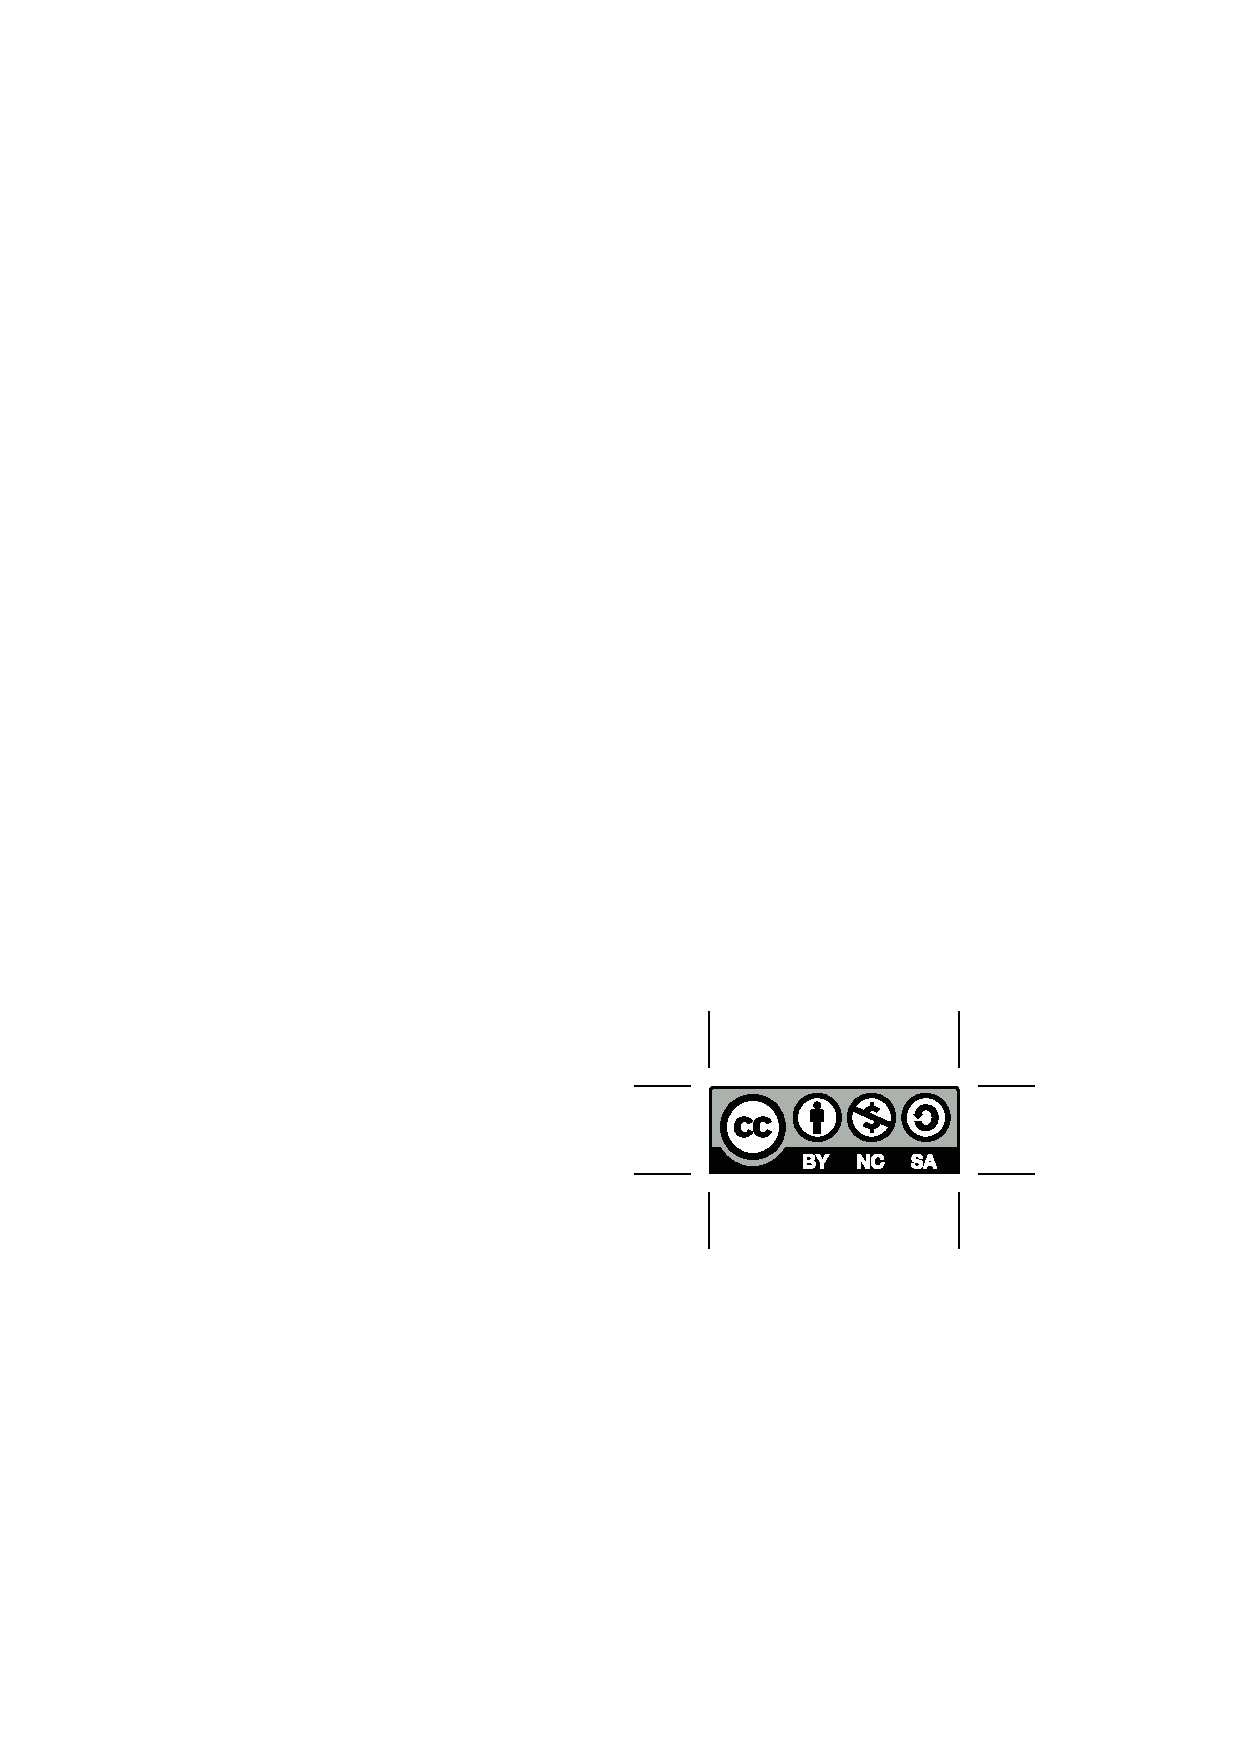
\includegraphics[height=1.5em]{by-nc-sa}}
Gautam Iyer, 2017.
\bigskip

\copyright{} 2017 by Gautam Iyer.
This work is licensed under the \emph{Creative Commons Attribution - Non Commercial - Share Alike 4.0 International License.}
This means you may adapt and or redistribute this document \textbf{for non commercial purposes}, provided you give appropriate credit and re-distribute your work under the same licence.
%In particular, you may edit these notes, and redistribute your modifications, provided you do so under the same licence.
%If, however, you would like to use material in these notes for a commercial purposes (e.g.\ in a book), you must obtain written prior approval.
To view the full terms of this license, visit
%\begin{center}
  \url{http://creativecommons.org/licenses/by-nc-sa/4.0/}
%\end{center}
or send a letter to Creative Commons, PO Box 1866, Mountain View, CA 94042, USA.

A DRM free PDF of these notes will always be available free of charge at \url{http://www.math.cmu.edu/~gautam}\,.
A self published print version at nominal cost may be made available for convenience.
The \LaTeX\ source is currently publicly hosted at GitLab: \url{https://gitlab.com/gi1242/cmu-mscf-944}\,.
%You are free to modify these notes under the terms of the licence.
%In particular, if you modify these notes the licence terms requires you to share your modifications (and \LaTeX\ source) under the same licence.
%In short, this means you must provide credit, share your work (including the \LaTeX\ source) under the same licence, and you may \textbf{not} use these notes for commercial purposes.
\bigskip

These notes are provided as is, without any warranty and Carnegie Mellon University, the Department of Mathematical-Sciences, nor any of the authors are liable for any errors.

\vspace{\stretch{3}}
\endgroup

\chapter*{Preface}

The purpose of these notes is to provide a rapid introduction to the Black-Scholes formula and the mathematics techniques used in this context.
Most mathematical concepts used are explained and motivated, but the complete rigorous proofs are beyond the scope of these notes.
These notes were written in 2017 when I was teaching a seven week course in the Masters in Computational Finance program at Carnegie Mellon University.

The notes are somewhat minimal and mainly include material that was covered during the lectures itself.
Only two sets of problems are included.
These are problems that were used as a review for the midterm and final respectively.
Supplementary problems and exams can be found on the course website:
  \url{http://www.math.cmu.edu/~gautam/sj/teaching/2016-17/944-scalc-finance1}\,.

For more comprehensive references and exercises, I recommend:
\begin{enumerate}
  \item
    \emph{Stochastic Calculus for Finance II} by Steven Shreve.
  \item 
    \emph{\href{http://bass.math.uconn.edu/finlmath.pdf}{The basics of Financial Mathematics}} by Rich Bass.
  \item
    \emph{Introduction to Stochastic Calculus with Applications} by Fima C Klebaner.
\end{enumerate}

%\setcounter{tocdepth}{2}
\tableofcontents\thispagestyle{empty}
\mainmatter
\hypersetup{pageanchor=true}
\end{document}
